\section{Related Work}

\subsection{3D Part Segmentation}
% \paragraph{3D Part Segmentation}
% Traditional 3D part segmentation
Traditional 3D part segmentation is typically cast as supervised semantic labeling on points or faces, using fixed part taxonomies provided by curated 3D segmentation datasets~\cite{partnet,3dmeshsegmentation,scannet,pointnet}.
%
Concretely, these methods~\cite{pointnet,pointtransformerv2,pointtransformerv3,pointpromptraining,meshcnn,meshtransformer} typically combine a 3D feature encoder with a segmentation head to predict dataset-specific part IDs.
%
However, the closed-world nature of both the label space and the training data limits generalization, making it difficult to transfer to unseen object categories or arbitrary, non-canonical part decompositions.


To alleviate this generalization bottleneck, recent works exploit 2D foundation models as transferable priors~\cite{clip,glip,sam,sam2,dino,dinov2} for 3D part segmentation.
%
A common strategy adopts a render-and-lift pipeline: it segments multi-view renderings with promptable 2D models and then projects and fuses the masks back onto the 3D surface~\cite{segmentanymesh,sam3d,sampro3d,partslip++,zerops}.
%
Despite being straightforward, this pipeline is often limited by incomplete view coverage and cross-view inconsistencies, which can lead to imprecise or blurred part boundaries after 2D-to-3D aggregation. 
%
Another line leverages distillation or feature projection to supervise 3D predictors with transferred 2D representations or pseudo-labels~\cite{partdistill,3dpartsegvia2dfea}; 
%
however, it still inherits the 2D--3D domain gap and multi-view alignment issues, and typically entails longer optimization and training cycles.


Recognizing the scalability and reliability issues of 2D-to-3D lifting, recent studies have shifted toward native feed-forward 3D segmentation that predicts masks directly on 3D representations at inference time.
%
Representative efforts for open-world part segmentation include training queryable 3D predictors with automatically curated supervision~\cite{find3d}, 
learning continuous part-aware 3D feature fields for direct decomposition~\cite{partfield}, 
and prompt-guided 3D mask prediction models~\cite{pointsam}, 
with more recent large-scale native 3D part segmentation models such as P3-SAM~\cite{p3sam} and PartSAM~\cite{partsam} further scaling training on millions of shape--part pairs. 
%
Despite encouraging progress, 
these native 3D approaches are fundamentally bottlenecked by the availability of large-scale, high-quality 3D part annotations, 
and the inconsistency of part taxonomies and granularity across datasets often introduces supervision mismatch, ultimately weakening cross-domain generalization.


\begin{figure*}
  \centering
  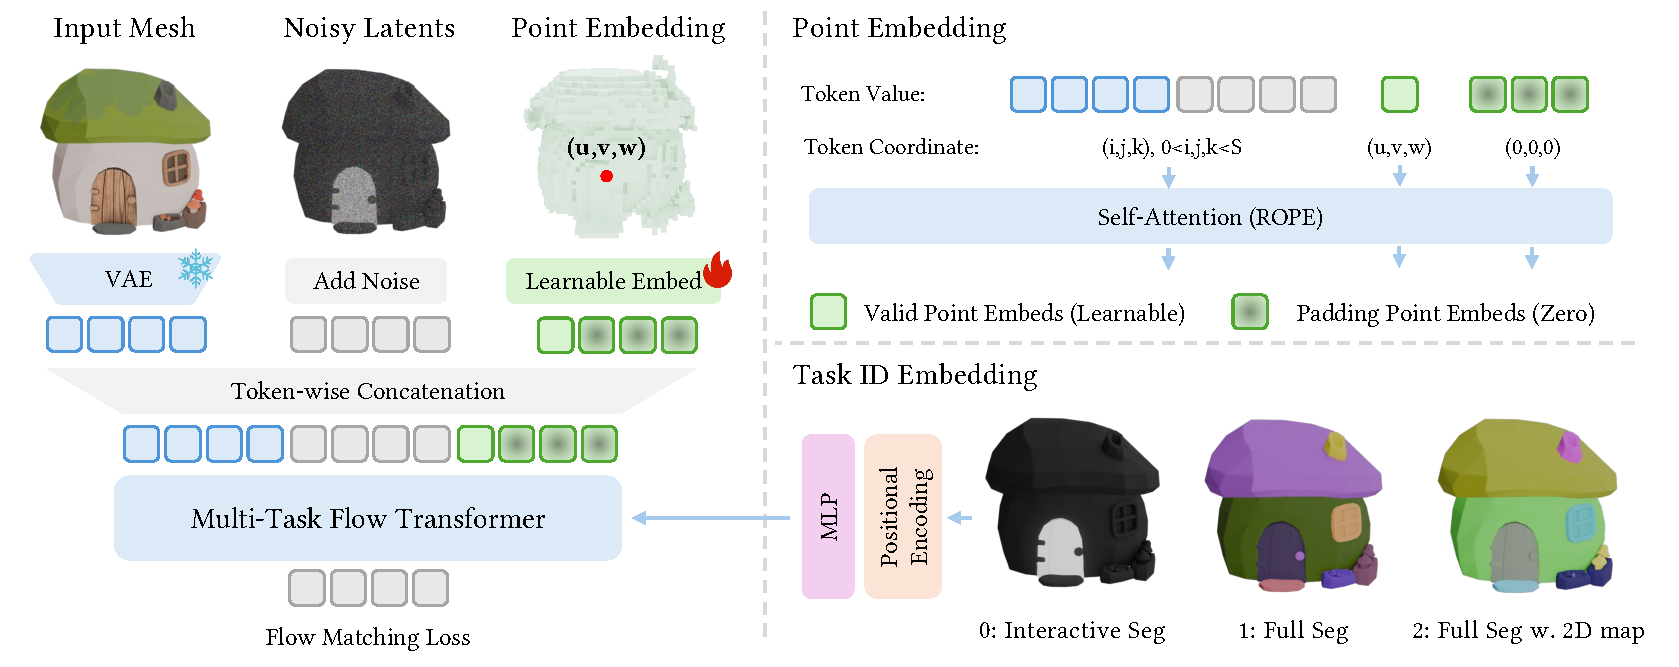
\includegraphics[width=\linewidth]{img/pipeline.pdf}
  \caption{
  Pipeline of \textit{SegviGen}. 
  %
  We reformulate 3D part segmentation as a conditional colorization task. 
  %
  During training, given a 3D mesh and its part-color ground truth, we encode both with a pretrained 3D VAE, add noise to the ground-truth latent, and then concatenate the geometry latent, noisy color latent, and point-condition tokens to form the final latent input.
  %
  Conditioned on the sampled timestep and a task embedding, the multi-task flow transformer predicts the noise residual for flow-matching training.
  }
  \label{fig:pipeline}
\end{figure*}

% \paragraph{3D Generative Model} 
\subsection{3D Generative Model}
The rapid progress of diffusion-based generative models~\cite{ho2020ddpm,song2020ddim}, together with the emergence of large-scale, high-quality 3D data collections~\cite{deitke2023objaverse,deitke2024objaversexl}, has catalyzed a wave of 3D generative methods~\cite{liu2024one2345,liu2023syncdreamer,long2024wonder3d,hong2023lrm,tang2025lgm,huang2024epidiff,zhang2024clay,wu2024unique3d,li2024craftsman,wen2024ouroboros3d,xu2024instantmesh,voleti2025sv3d,wang2024crm,liu2024one2345++,wu2024direct3d,zhao2024michelangelo,roessle2024l3dg,wu2024blockfusion,meng2024lt3sd,liu2024part123,dong2025tela,chen2024meshxlneuralcoordinatefield,chen2024meshanythingartistcreatedmeshgeneration,wang2024llamameshunifying3dmesh,hao2024meshtronhighfidelityartistlike3d,he2024neurallightrigunlockingaccurate,gao2025meshartgeneratingarticulatedmeshes,zhao2025deepmeshautoregressiveartistmeshcreation,wei2025octgptoctreebasedmultiscaleautoregressive,li2025step1x3dhighfidelitycontrollablegeneration,ye2025shapellmomninativemultimodalllm}.
A prevalent route builds 3D assets through a 2D-to-3D pipeline: models first synthesize multi-view imagery and subsequently reconstruct the 3D geometry and appearance from these views
~\cite{liu2023syncdreamer,long2024wonder3d,tang2025lgm,wen2024ouroboros3d,xu2024instantmesh,wang2024crm,voleti2025sv3d,huang2024mvadapter,qu2025deocc1to33ddeocclusionsingle,huang2025stereogsmultiviewstereovision}, yet view-to-view discrepancies in the synthesized images can propagate and degrade the final 3D quality.

In contrast, a growing family of native 3D generative models learns directly in 3D latent spaces, typically pairing a variational autoencoder~\cite{kingma2013vae} with a diffusion transformer (DiT)~\cite{peebles2023dit} to perform denoising over compact latents
~\cite{zhang2024clay,li2024craftsman,wu2024direct3d,zhao2024michelangelo,li2025triposg,chen2025ultra3defficienthighfidelity3d,dong2025morecontextuallatents3d,zhao2025assemblerscalable3dassembly,tang2025efficientpartlevel3dobject,lin2025partcrafterstructured3dmesh,wu2025dipodualstateimagescontrolled,wu2025direct3ds2gigascale3dgeneration,li2025triposghighfidelity3dshape,trellis,li2025craftsman3dhighfidelitymeshgeneration,trellis2}.
By learning to generate in a compact yet expressive 3D latent space, these models encode rich structural and texture knowledge across large-scale 3D assets, providing a strong transferable prior for downstream 3D part segmentation.
In particular, TRELLIS2~\cite{trellis2} introduces a field-free structured latent via an omni-voxel sparse voxel representation (O-Voxel) that jointly models geometry and appearance, enabling efficient generation with sharp, high-frequency textures that better preserve fine-grained part boundaries for 3D segmentation.